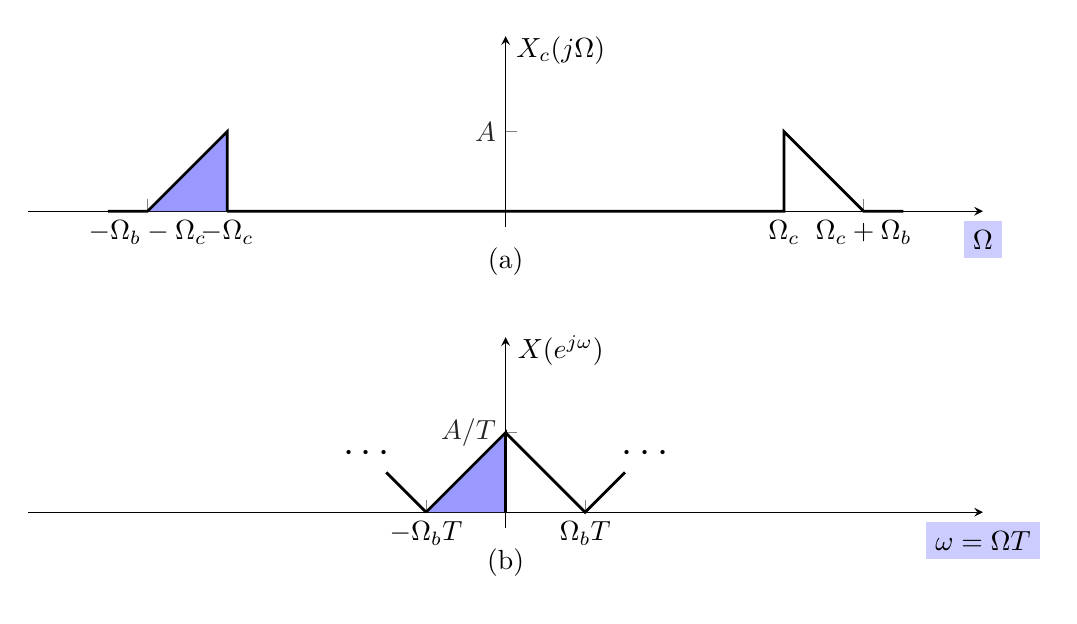
\begin{tikzpicture}
\begin{axis}[
	name=plot1,
	axis lines*=middle,
	enlargelimits = true,
	clip=true,
	scale only axis,
	width=\textwidth,
	height=0.2\textwidth,
	ymin=0, ymax=2,
	xmin=-10, xmax=10,
	axis line style={->,>=stealth},
	xlabel={ \tikz[baseline]{\node[fill=blue!20,anchor=base] (t1) {$\Omega$};}},
	ylabel={ $X_c(j\Omega)$},
	every axis x label/.style={
		at={(ticklabel* cs:1)},
		anchor=north,
	},
	every axis y label/.style={
		at={(ticklabel* cs:0.8)},
		anchor=south,
		xshift=0.7cm,
	},	
	ytick=1,
	yticklabels={ $A$},
	xtick={-9, -7, 0, 7, 9},
	xticklabels={ $-\Omega_b-\Omega_c$,  $-\Omega_c$,  0,  $\Omega_c$,  $\Omega_c+\Omega_b$}, 
	every outer y axis line/.append style={white!15!black},
	every y tick label/.append style={font=\color{white!15!black}},
	legend style={draw=white!15!black,fill=white,legend cell align=left}]
	\addplot[solid, line width=1pt] coordinates {(-7, 0) (7, 0) (7, 1) (9, 0) (10, 0)};
    \addplot[solid, fill=blue!40, line width=1pt] coordinates {(-10, 0) (-9, 0) (-7, 1) (-7, 0)};
\end{axis}

\begin{axis}[
	name=plot2,
    at=(plot1.below south east), anchor=above north east, yshift=-0.75cm,
	axis lines*=middle,
	enlargelimits = true,
	clip=true,
	scale only axis,
	width=\textwidth,
	height=0.2\textwidth,
	ymin=0, ymax=2,
	xmin=-10, xmax=10,
	axis line style={->,>=stealth},
	xlabel={ \tikz[baseline]{\node[fill=blue!20,anchor=base] (t1) {$\omega = \Omega T$};}},
	ylabel={ $X(e^{j\omega})$},
	every axis x label/.style={
		at={(ticklabel* cs:1)},
		anchor=north,
	},
	every axis y label/.style={
		at={(ticklabel* cs:0.8)},
		anchor=south,
		xshift=0.7cm,
	},	
	ytick=1,
	yticklabels={ $A/T$},
	xtick={-2, 2},
	xticklabels={ $-\Omega_bT$,  $\Omega_bT$}, 
	every outer y axis line/.append style={white!15!black},
	every y tick label/.append style={font=\color{white!15!black}},
	legend style={draw=white!15!black,fill=white,legend cell align=left}]
	\addplot[solid, line width=1pt] coordinates {(0, 1) (2, 0) (3, 0.5)};
    \addplot[solid, fill=blue!40, line width=1pt] coordinates {(-2, 0) (0, 1) (0, 0)};
    
    \addplot[solid, line width=1pt] coordinates {(-3, 0.5) (-2, 0)};
    \node[above] at (axis cs: -3.5, 0.5) {\Large $\cdots$};
    \node[above] at (axis cs: 3.5, 0.5) {\Large $\cdots$};
\end{axis}
\node[below, inner sep=0.25cm] at (plot1.south) {(a)};
\node[below, inner sep=0.25cm] at (plot2.south) {(b)};

\end{tikzpicture}
